\documentclass{slide}
% \usepackage{pgfpages}

%\setbeameroption{show notes on second screen}

\usepackage{tikz}
\usetikzlibrary{backgrounds}
\usetikzlibrary{shapes}
\usetikzlibrary{tikzmark}
\usetikzlibrary{calc}
\usetikzlibrary{positioning}
\usetikzlibrary{arrows}
\usetikzlibrary{fit}

\title{Containers}
\subtitle{Software Architecture}
\author{Brae Webb}
\date{\week{3}}

\usepackage{languages}

\newcommand{\commandnoarg}[2]{
\begin{frame}
    \bash{#1}
    {\color{primary}Summary}

    #2
\end{frame}
}

\newcommand{\command}[3]{
\begin{frame}
    \bash{#1}
    {\color{primary}Summary}

    #2
    \vspace{1em}

    {\color{primary}Key parameters}
    \begin{description}
        #3
    \end{description}
\end{frame}
}

\titlegraphic{
    \begin{tikzpicture}[overlay,remember picture]
    \node[left=0.1cm] at (current page.0){
        
\includegraphics[width=8cm]{images/docker}
    };
    \end{tikzpicture}
}

\begin{document}

\maketitle

\questionanswer{What is a \highlight{container}?}{
A way of \highlight{packaging software} and its dependencies such that the software can be run in numerous environments.
}

\point[Okay...]{How hard could that be?}

\begin{frame}[fragile]{Packaging software}
    \vspace{-1em}
    \begin{code}[language=python]{program.py}
#!/usr/bin/env python3

import numpy as np
import re

my_arr = np.array([5, 2, 9, 7, 3])
max_element = np.max(my_arr)

duplicated_max = re.sub(".*", f"{max_element}", "X")
print(sum(int(x) for x in duplicated_max))
    \end{code}
    \begin{code}[numbers=none]{}
> ./program.py
18
    \end{code}
\end{frame}

\point[demo]{Transferring this software to client.}

\begin{frame}[fragile]
    \begin{code}[numbers=none]{}
> ./program.py
/usr/bin/env: 'python3': No such file or directory
    \end{code}
    \pause
    No Python interpreter installed,
    have to install Python and all it's dependencies.
\end{frame}

\begin{frame}[fragile]
    \begin{code}[numbers=none]{}
> ./program.py
File "./program.py", line 9
    duplicated_max = re.sub(".*", f"{max_element}", "X")
                                                 ^
SyntaxError: invalid syntax
    \end{code}
    \pause
    f-strings aren't supported in Python 3.5!
    Have to upgrade to Python 3.6.
\end{frame}

\begin{frame}[fragile]
    \begin{code}[numbers=none]{}
> ./program.py
Traceback (most recent call last):
  File "./program.py", line 3, in <module>
    import numpy as np
ModuleNotFoundError: No module named 'numpy'
    \end{code}
    \pause
    A Python dependency used by our code isn't installed.
    Have to install numpy (hopefully the right version...).
\end{frame}

\begin{frame}[fragile]
    \begin{code}[numbers=none]{}
> ./program.py
9
    \end{code}
    \pause
    ???
\end{frame}

\question{Not so easy... what do we need?}

\begin{frame}
    \vspace{-2em}
    \begin{columns}
    \begin{column}{0.4\textwidth}
    {\color{primary}\large A wall}
    \vspace{1em}

    A big wall around our environment so that we
    \highlight{know what software} we are actually depending upon.
    \end{column}
    \begin{column}{0.6\textwidth}
    \begin{center}
    
\includegraphics[height=0.95\textheight]{images/python-wall}
    \end{center}
    \end{column}
    \end{columns}
\end{frame}

\begin{frame}
    \vspace{-2em}
    \begin{columns}
    \begin{column}{0.6\textwidth}
    \begin{center}
    
\includegraphics[height=0.95\textheight]{images/packaging}
    \end{center}
    \end{column}

    \begin{column}{0.4\textwidth}
    {\color{primary}\large A package}
    \vspace{1em}

    A way to box up all your software and dependencies
    so that it can be \highlight{transferred} and \highlight{run} in a different environment.
    \end{column}
    \end{columns}
\end{frame}

\section{A History of Containers %
\footnote{This is a very Linux focused history --- container technology also exists in the Windows world.}}

\begin{frame}{1979}
    \vspace{-3em}
    \begin{columns}
    \begin{column}{0.5\textwidth}
    {\color{primary}\Large Unix Version 7}
    \vspace{1em}

    \large Introducing... \highlight{chroot}
    \end{column}
    \begin{column}{0.5\textwidth}
    \begin{center}
    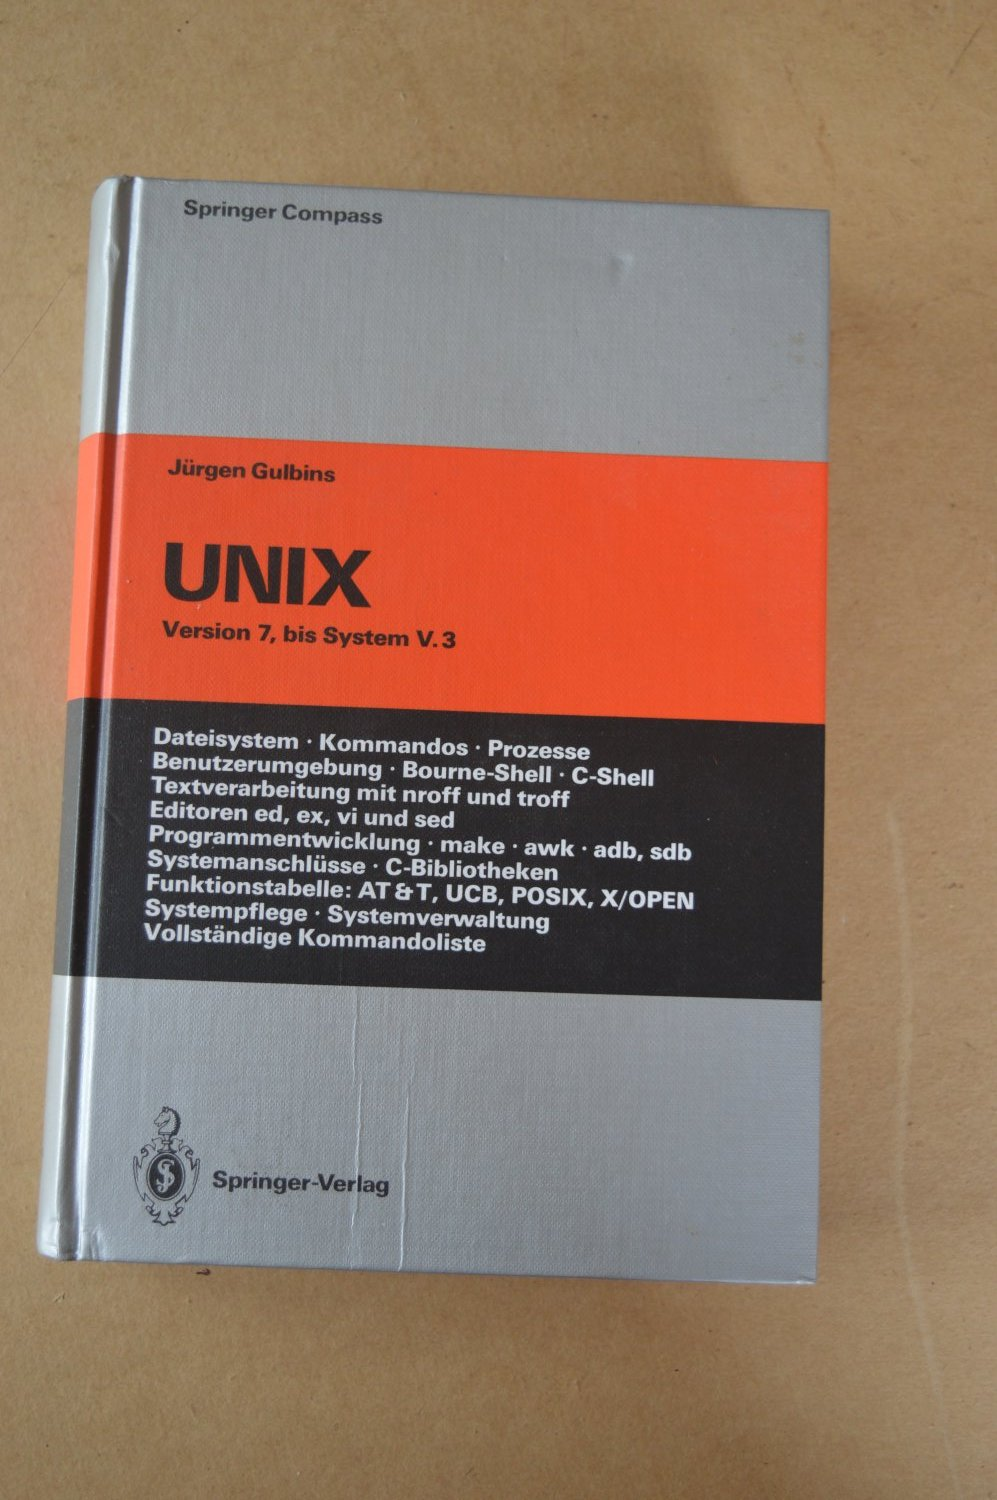
\includegraphics[height=0.95\textheight]{images/unix7}
    \end{center}
    \end{column}
    \end{columns}
\end{frame}

\point[demo]{Exploring \highlight{chroot}}

\begin{frame}[fragile]{Exploring \highlight{chroot}}
    \begin{code}[numbers=none]{}
> mkdir ./jail
> cd jail
> chroot . /bin/ls
chroot: failed to run command '/bin/ls': No such file or directory
> mkdir bin
> cp /bin/ls bin
> chroot . /bin/ls
chroot: failed to run command '/bin/ls': No such file or directory
    \end{code}
\end{frame}
\note[itemize]{
    \item First chroot -- Doesn't exist from our new root.
    \item Second chroot -- Exists but it can't find files on which ls depends.
}

\begin{frame}[fragile]{Exploring \highlight{chroot}}
    \vspace{-0.5em}
    \begin{code}[numbers=none]{}
> ldd /bin/ls
    libselinux.so.1 => /lib/x86_64-linux-gnu/libselinux.so.1 (0x00007f0097135000)
    libc.so.6 => /lib/x86_64-linux-gnu/libc.so.6 (0x00007f0096f0d000)
    libpcre2-8.so.0 => /lib/x86_64-linux-gnu/libpcre2-8.so.0 (0x00007f0096e76000)
    /lib64/ld-linux-x86-64.so.2 (0x00007f0097189000)
> cp --parents /lib/x86_64-linux-gnu/libselinux.so.1 /lib/x86_64-linux-gnu/libc.so.6 /lib/x86_64-linux-gnu/libpcre2-8.so.0 /lib64/ld-linux-x86-64.so.2 .
> ls
bin  lib  lib64
> ls lib/x86_64-linux-gnu/
libc.so.6  libpcre2-8.so.0  libselinux.so.1
    \end{code}
\end{frame}

\begin{frame}[fragile]{Exploring \highlight{chroot}}
    \begin{code}[numbers=none]{}
> chroot . /bin/ls
bin  lib  lib64
> chroot . /bin/ls /
bin  lib  lib64
> chroot . /bin/ls ..
bin  lib  lib64
> chroot . /bin/ls /bin
ls
    \end{code}
\end{frame}
\note[itemize]{
    \item ldd -- Lists dependencies
    \item cp -- Copy dependencies
    \item ls -- Show that these are now within our directory.
}

\begin{frame}[fragile]{Chroot Limitations}
    {\LARGE
    \begin{itemize}
        \item \highlight{Only filesystem isolation}
        \begin{itemize}
            \Large \item processes, network, etc. still accessible
        \end{itemize}
        \item Not very \highlight{user friendly}
        \item Not very \highlight{portable}
        \item \highlight{Jailbreak} is possible
    \end{itemize}
    }
\end{frame}
\note[itemize]{
    \item Can now run chroot . /bin/ls -- Everything is available from new root.
    \item Second chroot -- Shows that it considers our directory to be the root.
    \item Third chroot -- Shows we can't go to a parent directory.
}


\begin{frame}{1992}
    \begin{columns}
    \begin{column}{0.8\textwidth}
    \begin{center}
    \href{https://www.bell-labs.com/institute/blog/plan-9-bell-labs-cyberspace/}{
    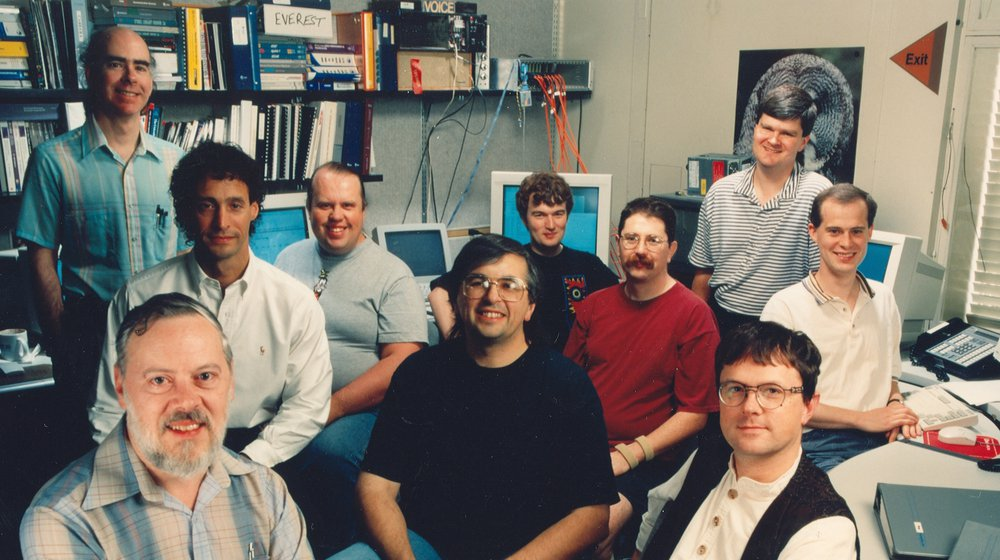
\includegraphics[width=\textwidth]{images/plan9}
}
\note[itemize]{
    \item Image shows members of the Bell Labs Computing Techniques Research Department, which developed Plan 9:
    \item (foreground, from left) Dennis Ritchie, Dave Presotto, Rob Pike,
    \item (background, from left) Tom Killian, Allen Eisdorfer, Tom Duff, Phil Winterbottom, Jim McKie, Howard Trickey and Sean Dorward.
}
    \end{center}
    \end{column}
     \begin{column}{0.25\textwidth}
    {\color{primary}\Large Plan 9}
    \vspace{1em}

    \large Introducing... \highlight{layered filesystem}
    \end{column}

    \end{columns}

\end{frame}

\point[Layered filesystem]{
    \begin{itemize}
        \item Projection on \highlight{read}
        \item Copy on \highlight{write}
    \end{itemize}
}

%%%%%%%%%%%%%%%%%%%%%%%%%%%%%%%%%%%%%%%%%%%%%%%%%%%%%%%%%%%%%%%%%%%%%%%%%%%%%%%%%%%%%%%%%%%%%%%%%%%%%%%%%%%%%%
%
% DELETED SECTION
%
%%%%%%%%%%%%%%%%%%%%%%%%%%%%%%%%%%%%%%%%%%%%%%%%%%%%%%%%%%%%%%%%%%%%%%%%%%%%%%%%%%%%%%%%%%%%%%%%%%%%%%%%%%%%%%

\begin{frame}{In the practical this week...}
    \centering
    
\includegraphics[width=.95\textwidth]{images/practical}
\end{frame}


\begin{frame}
    \centering
\href{https://xkcd.com/1988/}{
    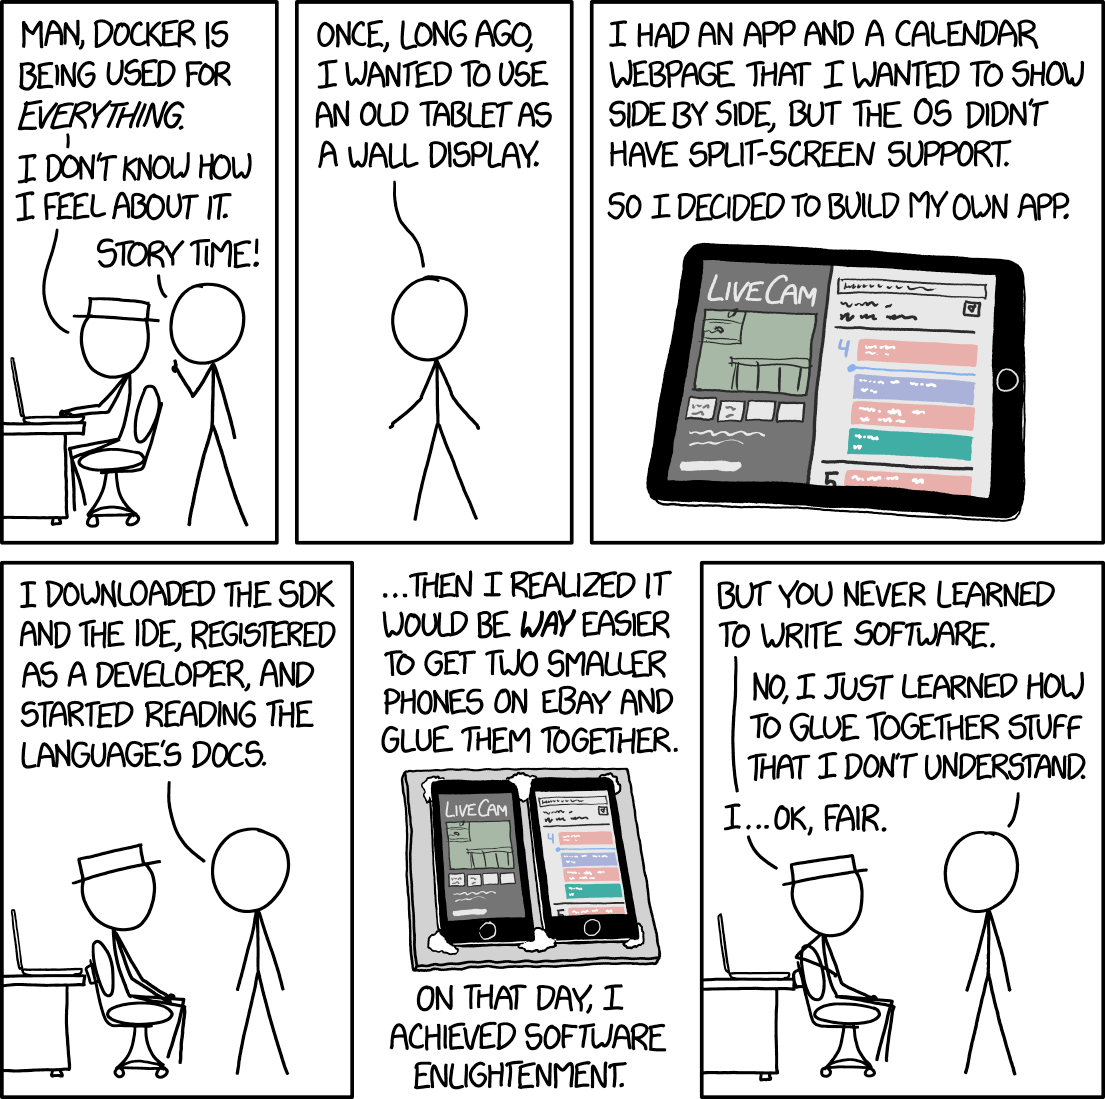
\includegraphics[height=0.9\textheight]{./images/xkcd1988}
}

\url{https://xkcd.com/1988/}
\end{frame}


% \references{articles,books}

\end{document}
